\section{Diseño Tolerante a Fallas de Hardware}

\subsection{Introducción al Análisis de Tolerancia a Fallas}\label{subsec:introduccion_al_analisis_de_tolerancia_a_fallas}

En los últimos años se ha incrementado mucho la presencia de UAVs en espacio aéreo civil. Debido a esto, se plantea que los UAVs deberían presentar características que permitan un funcionamiento correcto, tolerante a fallas. Como consecuencias posibles, el hecho de volar en espacio aéreo civil puede llegar a causar daño físico a personas, si es que un vehículo presenta una falla y por ejemplo pierde el control. Otra de las posibles consecuencias tiene que ver con los costos que puede ocasionar una falla en una misión relacionada a una actividad laboral. El hecho de tener que repetir la misión puede traer mayores costos para la actividad en cuestión.

El objetivo del diseño tolerante a fallas consiste en mejorar la confianza (\textit{Dependability}) del sistema, apuntando a que este pueda seguir ejecutando su función de manera correcta a pesar de la presencia de una cierta cantidad de fallas \cite{nelson1990fault}. De esta última expresión se puede tomar una definición de lo que es un sistema tolerante a fallas.

\begin{mydef}
    \textbf{Sistema Tolerante a Fallas:} es aquel donde una falla no implica necesariamente un error en el funcionamiento. Un sistema tolerante a fallas no es aquel donde no ocurren fallas, sino que más bien, se acepta que las fallas pueden ocurrir en el sistema, pero lo que se pretende es que el sistema pueda cumplir con su función de igual manera.
\end{mydef}

De manera de introducir la nomenclatura que se encuentra en la bibliografía \cite{nelson1990fault}, se definen los siguientes términos:

\begin{itemize}
    \item Falla (\textit{Fault}): es alguna condición anómala, no esperada.
    \item Error: un error ocurre cuando una falla se manifiesta y produce un comportamiento fuera de lo esperado en alguna parte del sistema.
    \item Fracaso (\textit{Failure}): quiere decir que el sistema no puede cumplir con su función de manera adecuada.
\end{itemize}

Una de las formas de cuantificar la confianza es a través de la fiabilidad del sistema (\textit{Reliability}). Esta se expresa en la ecuación \eqref{eq:Reliability}, y se define como la probabilidad de que el sistema pueda cumplir su función de manera correcta en un intervalo de tiempo $[t_0;t]$, dado que en el instante inicial $t_0$ el sistema podía hacerlo.

\begin{equation}
    R(t) = \mathtt{P}\left( \text{funcionamiento correcto en $t$} | \text{funcionamiento correcto en $t_0$} \right)
    \label{eq:Reliability}
\end{equation}

Dado que en el intervalo $[t_0;t]$ puede o no ocurrir una falla, la probabilidad de que el sistema pueda cumplir su función en $t$ puede expresarse como en la ecuación \eqref{eq:Reliability_2}. Si no ocurre ninguna falla, luego el sistema podrá seguir cumpliendo su función en $t$. Además, si llegase a ocurrir una falla, pero el sistema tiene la capacidad de tolerarla, luego el sistema de igual manera podrá seguir cumpliendo su función en el instante $t$.

\begin{equation}
    \begin{aligned}
        R(t) &= \mathtt{P}\left( \text{no ocurrio una falla en $[t_0;t]$} \right)\\ &+ \mathtt{P}\left( \text{funcionamiento correcto en $t$}|\text{ocurrió una falla en $[t_0;t]$} \right) \ \mathtt{P}\left( \text{ocurrió una falla en $[t_0;t]$} \right)
    \end{aligned}
    \label{eq:Reliability_2}
\end{equation}

En el caso en el que se tuviera un sistema que no comprende ningún mecanismo de tolerancia a fallas, luego la fiabilidad sería exactamente igual a la probabilidad de que no ocurra una falla, ya que la ocurrencia de una falla causaría un funcionamiento incorrecto. Esto no necesariamente representa un problema. Si el sistema en cuestión es tal que puede demostrarse que la probabilidad de que no ocurra una falla es lo suficientemente alta, luego no se requeriría el uso de técnicas de tolerancia a fallas.

En un sistema donde no hay tolerancia a fallas, la fiabilidad quedaría definida como en la ecuación \eqref{eq:Reliability_3} y la única manera de mejorarla sería incrementando la probabilidad de que no ocurra ninguna falla en el intervalo $[t_0;t]$.

\begin{equation}
    R(t) = \mathtt{P}\left( \text{no ocurrio una falla en $[t_0;t]$} \right)
    \label{eq:Reliability_3}
\end{equation}

La manera de hacer esto puede ser por ejemplo, utilizando componentes o módulos de muy buena calidad, lo suficientemente confiables como para cumplir con los requerimientos de fiabilidad \cite{nelson1990fault}. Sin embargo, esto puede ser muy costoso, pensando en que un sistema puede tener una enorme cantidad de posibles fallas. No solo eso, sino que esto dificulta la etapa de diseño de un sistema, ya que cualquier error de diseño que no se haya tenido en cuenta puede llegar a causar una falla y por ende un fracaso del sistema. Por el contrario, la tolerancia a fallas plantea permitir que las fallas existan, pero aplicando técnicas para tolerarlas.

Volviendo a la ecuación \eqref{eq:Reliability_2}, la probabilidad de que el sistema funcione correctamente a pesar de la falla, está pesada por la probabilidad de ocurrencia de dicha falla. A partir de esto se desprende que aplicar técnicas de tolerancia a fallas para cada una de las posibles fallas puede resultar exhaustivo, principalmente porque deberían conocerse todas las fallas posibles, además de ser algo costoso. Lo que se propone es considerar solo aquellas fallas cuya criticidad es alta.

A modo de ejemplo, una \textbf{falla en un sensor de la computadora de vuelo puede generar una lectura incorrecta}. En consecuencia, esto decantará en un \textbf{error, es decir, en un cálculo de la ley de control incorrecto}. Finalmente, este error puede llevar al \textbf{fracaso de la misión, por ejemplo si el vehículo no es capaz de seguir una trayectoria dada en tiempo y forma}. Esto da a entender que una falla en un sensor es crítica y que por ende requiere la aplicación de técnicas de tolerancia a fallas.

Aquí se habla de falla en un sensor como algo general. Un sensor podría fallar de muchas maneras y debido a muchas razones. Por ejemplo, puede dejar de funcionar por un defecto propio del componente, puede entregar lecturas erróneas debido a interferencias electromagnéticas, por efectos de la temperatura, falta de calibración, etc. Cada uno de estos requeriría la aplicación de un mecanismo tolerante a fallas.

\subsection{Causales de Fallas de Hardware y Modelo de Fallas Arbitrarias}

Uno de los métodos para aplicar mecanismos de tolerancia a fallas consiste en hacer un análisis de los posibles modos de falla. Un ejemplo es el del análisis \textit{Failure Modes and Effects Analysis} (FMEA). Este consiste en realizar un análisis exhaustivo de los posibles modos de falla más probables y sus posibles efectos en el sistema. En función de este análisis, se toman medidas para tolerar las fallas más críticas. El objetivo de este tipo de análisis suele ser demostrar ante alguna autoridad ceritifcante, que la confianza del sistema se mantiene por encima de cierto valor. Este tipo de análisis suele consumir mucho tiempo y esfuerzo, lo que se traduce en un mayor costo del desarrollo \cite{lala1994architectural}.

Una forma de alivianar esta tarea es la de considerar un modelo de falla de hardware más conservador, donde se asume que una falla de hardware consiste en que esta presente un comportamiento anómalo arbitrario, es decir, de cualquier tipo. A este tipo de comportamiento se lo denomina falla bizantina o \textit{Byzantine Fault} en inglés y básicamente consiste en asumir que el elemento que manifiesta la falla presenta un comportamiento arbitrario. Por ejemplo, un sensor puede dejar de funcionar repentinamente y no dar más respuesta, puede dejar de enviar respuesta por un período de tiempo y luego volver a funcionar, podría también enviar datos a un microcontrolador pero que esos datos sean incoherentes, etc. El modelo de falla bizantina no asume modos de falla, sino que el comportamiento es arbitrario \cite{roth2021not}\cite{hiergeist2017internal}\cite{lala1994architectural}. Se define un sistema tolerante a este tipo de fallas.

\begin{mydef}
    \textbf{Sistema Byzantine Resilient}: es aquel capaz de tolerar una cierta cantidad de fallas arbitrarias a la vez.
\end{mydef}

Dado que no se asume un modo de falla del hardware, no se requiere un análisis tan exhaustivo como el mencionado FMEA. Considerando el costo y esfuerzo que lleva realizar un análisis de modos de fallas, el hecho de poder contar con un sistema con las características que aquí se mencionan resulta atractivo para alivianar el trabajo relacionado a la validación del sistema tolerante a fallas en cuestión.

A priori, puede parecer que desarrollar un sistema tolerante a fallas arbitrarias representa un trabajo sumamente complejo. La manera de implementar un sistema tolerante a fallas bizantinas es a través del uso de redundancias. Este resultado se toma a partir de un problema teórico denominado \textit{The Byzantine Generals Problem} \cite{lamport2019byzantine}.

\subsection{Tolerancia a Fallas a Partir de Redundancias}

La principal técnica de tolerancia a fallas es el uso de redundancias \cite{nelson1990fault}\cite{prasad1989fault}\cite{lala1994architectural}. Esto quiere decir, que se replica el hardware en el sistema y cada réplica realiza la misma tarea en paralelo. De esta forma, si una de las réplicas presenta una falla (arbitraria por ejemplo), esta puede detectarse a partir de la comparación con las demás réplicas, o incluso pasar desapercibida. Utilizando la nomenclatura definida en la sección \ref{subsec:introduccion_al_analisis_de_tolerancia_a_fallas}, que una falla pase desapercibida quiere decir que no se manifiesta como un error, sino que esta es contenida. A continuación se presentan algunas arquitecturas redundantes para la tolerancia a fallas.

\subsubsection{Redundancia Doble}

Una arquitectura simple es la redundancia doble. En este tipo de sistemas, dos nodos de un sistema funcionan en paralelo y comparan sus resultados. La comparación permite detectar si los resultados difieren entre sí, lo que se traduce en que ocurrió un error.

\begin{figure}[H]
    \centering
    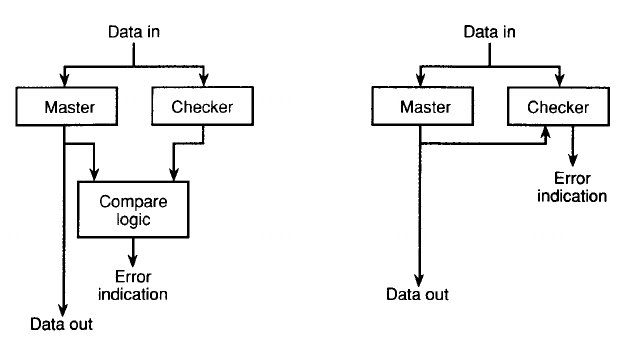
\includegraphics[width=0.6\textwidth]{img/3_4_lockstep_architecture.png}
    \caption{En la figura de la izquierda, dos sistemas ejecutan las mismas operaciones, mientras que otro sistema externo se encarga de compara las salidas de ambos para detectar errores. En la figura de la derecha, el bloque comparador se encuentra integrado en el sistema \textit{checker}. La imagen fue extraida de \cite{nelson1990fault}.}
    \label{fig:3_4_lockstep_architecture}
\end{figure}

Este tipo de arquitectura permite detectar si ocurrió un error, pero no permite identificar de qué nodo proviene el error. En la figura \ref{fig:3_4_lockstep_architecture} se muestran dos configuraciones. La configuración de la derecha puede ser implementada a través de dos CPUs totalmente independientes (a veces denominada \textit{Loosely-Synchronized Dual Processor Architecture}) o a través del uso de un procesador de dos núcleos, donde uno sería el \textit{Master} y otro el \textit{checker}\cite{baleani2003fault}. En esta última, ambos se encuentran sincronizados por estar en el mismo chip y compartir fuente de clock. En la figura \ref{fig:3_4_lockstep_architecture_2} se muestra un esquema de ambos casos.

\begin{figure}[H]
    \centering
    \begin{subfigure}[b]{0.49\textwidth}
        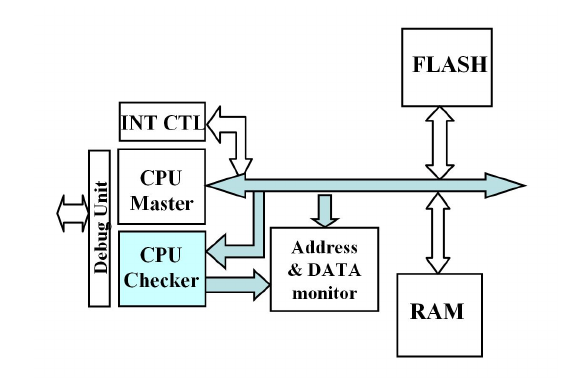
\includegraphics[width=\textwidth]{3_4_lockstep_dual_core.png}
        \caption{Lockstep dual processor architecture.}
        \label{fig:3_4_lockstep_dual_core}
    \end{subfigure}
    \begin{subfigure}[b]{0.49\textwidth}
        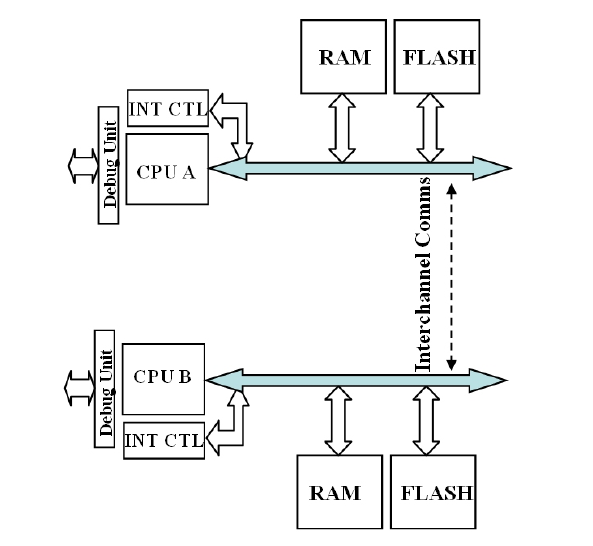
\includegraphics[width=\textwidth]{3_4_loosely_synchronized_dual_processor_architecture.png}
        \caption{Loosely synchronized dual processor architecture.}
        \label{fig:3_4_loosely_synchronized_dual_processor_architecture}
    \end{subfigure}
    \caption{Se muestran dos casos para un sistema con redundancia doble. La imagen fue extraida de \cite{baleani2003fault}.}
    \label{fig:3_4_lockstep_architecture_2}
\end{figure}

Debido a que no se puede saber cuál de las dos CPUs cometió el error, esta arquitectura plantea que en el caso en el que la comparación entre ambas CPUs genere una discrepancia en los resultados, cada una de ellas deben ejecutar un algoritmo interno, para detectar si ellas fueron las que cometieron el error o no. En \cite{zhang2015dual} y en \cite{SolanoPerez2019} se pueden encontrar un proyectos de redundancias doble para un UAV.

\subsubsection{Redundancia Triple}

Esta arquitectura puede encontrarse en la literatura con el nombre \textit{Triple Modular Redundant (TMR) Architecture} \cite{baleani2003fault}\cite{nelson1990fault}\cite{prasad1989fault}. Esta arquitectura consiste en utilizar tres computadoras en paralelo, las cuales computan los mismos resultados. Luego, se comparan los resultados. Se asume que solamente 1 de las 3 presentará una falla a la vez. En dicho caso, los resultados de dos computadoras serán iguales y la de la tercera será distinto, por lo que solamente se descarta el resultado erróneo. En la figura \ref{fig:3_5_TMR} se muestra un diagrama con la arquitectura TMR. Una diferencia de esta arquitectura respecto de la doble redundancia, es el hecho de que puede detectarse cuál de las computadoras falló y además, no es necesario que todas las computadoras ejecuten una rutina para verificar si cometieron el error o no. Esto resulta especialmente útil en sistemas de tiempo real, donde no puede detenerse el sistema para realizar una verificación interna. Esto se denomina \textit{Fault Masking}.

\begin{figure}[H]
    \centering
    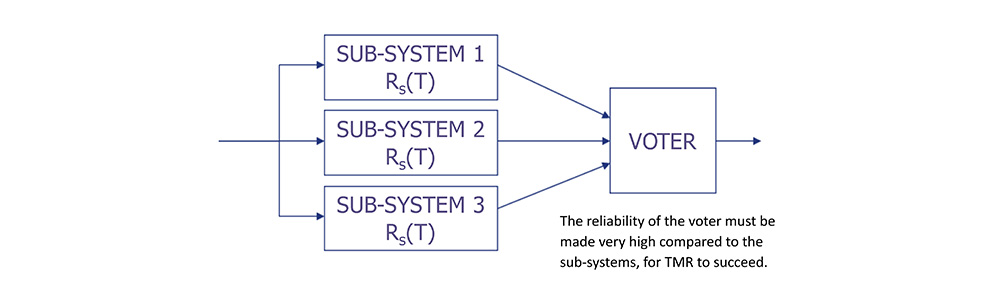
\includegraphics[width=0.8\textwidth]{3_5_TMR.png}
    \caption{Arquitectura TMR. La imagen fue extraida de \cite{TMRwebPage}.}
    \label{fig:3_5_TMR}
\end{figure}

Como indica el texto de la imagen, una cuestión clave de esta arquitectura es el bloque denominado \textit{VOTER}. Debido a que este bloque es el que determina cuál es el resultado correcto, se requiere que la fiabilidad, $R(t)$, de este sea mucho mayor que la de cada computadora de vuelo. Esto se logra a través del uso de hardware más robusto, lo que resulta en que el bloque \textit{VOTER} sea más costos que cada computadora de vuelo. Por ejemplo, cada computadora de vuelo puede comprender un microcontrolador COTS, mientras que el bloque voter puede estar implementado con un ASIC específico para esa aplicación \cite{hiergeist2017internal}. Si bien este bloque tiene una fiabilidad mucho mayor, siempre existe la probabilidad de que ocurra un error en este. En cuyo caso, el error puede decantar en un fracaso, por ejemplo si el \textit{VOTER} elige como resultado correcto, aquel que realmente no lo era.

\begin{mydef}
    \textbf{Single-Point Failure}: si la arquitectura del sistema es tal que una parte del sistema X fracasa en cumplir su trabajo dentro del sistema, luego el sistema completo fracasará en cumplir su función. En dicho caso, X es un punto único de falla.
\end{mydef}

Una forma de combatir esto es replicar los bloques que realizan la votación \cite{nelson1990fault}. De esta manera, también pueden enmascararse errores de los bloques que realizan la votación.

\subsection{Algunos Requerimientos de un Sistema Redundante}

Si bien el uso de redundancias apunta a incrementar la fiabilidad del sistema y tolerar fallas, es un error pensar que el simple hecho de tener un sistema redundante equivale a un incremento de la fiabilidad \cite{lala1994architectural}. Esto es principalmente por el hecho de que un sistema redundante incluye además las comunicaciones y rutinas necesarias para ejecutar las votaciones. Si estas funcionalidades no son administradas de manera correcta, un sistema redundante solamente solo traerá más fallas.

\subsubsection{Sincronismo de los Nodos}

En las arquitecturas antes presentadas, se menciona que se realiza una comparación de los resultados calculados por cada nodo, para detectar/enmascarar errores. Para que el funcionamiento de esta comparación sea adecuado, los nodos deben estar sincronizados. Esto es un requerimiento para sistemas de tiempo real, como el caso de la computadora de vuelo de un UAV.

En la figura \ref{fig:3_4_1_sincronizacion} se muestra un ejemplo. En el instante $t$, se presenta una nueva medición de un sensor a las tres computadoras de vuelo. Al comienzo de la misión, todas ellas estarán sincronizadas y generán un resultado del cálculo de la ley de control que corresponde al mismo intervalo de tiempo. Luego se realiza la votación para elegir el valor correcto. La figura \ref{fig:3_4_1_sincronizacion_2}, muestra lo que sucede al cabo de un período de tiempo. Se presenta una nueva medición de un sensor en el instante $t$. Debido a la desincronización, es posible que las computadoras de vuelo no presenten sus resultados al \textit{Voter} a tiempo. Este caso suele estar contemplado dentro de las posibilidades y correpsonde al caso en el que una computadora de vuelo presentó un error y debido a ello no respondió con ningún valor (por ejemplo, se reinició su procesador debido a un \textit{watchdog}).

\begin{figure}[H]
    \centering
    \begin{subfigure}[b]{0.49\textwidth}
        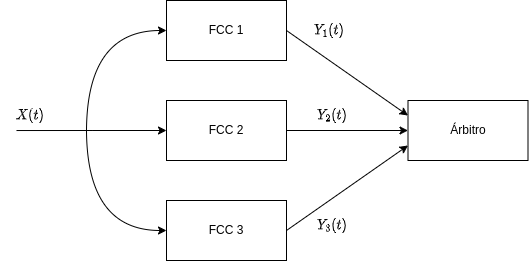
\includegraphics[width=\textwidth]{img/3_4_1_sincronizacion_1.png}
        \caption{Computadoras de vuelo al inicio de la misión.}
        \label{fig:3_4_1_sincronizacion_1}
    \end{subfigure}
    \begin{subfigure}[b]{0.49\textwidth}
        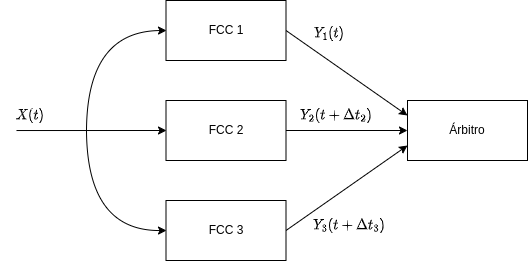
\includegraphics[width=\textwidth]{img/3_4_1_sincronizacion_2.png}
        \caption{Al cabo de un período de tiempo, se desincronizarán.}
        \label{fig:3_4_1_sincronizacion_2}
    \end{subfigure}
    \caption{Al cabo de un rato, la desincronización entre FCCs impactará en el sistema redundante.}
    \label{fig:3_4_1_sincronizacion}
\end{figure}

Otra cosa que puede suceder, es que los resultados propuestos por las computadoras de vuelo, $Y_1$, $Y_2$ e $Y_3$ correspondan a intervalos de tiempo distintos. Este caso es todavía peor que el anterior, ya que no se encuentra contemplado. 

\begin{figure}[H]
    \centering
    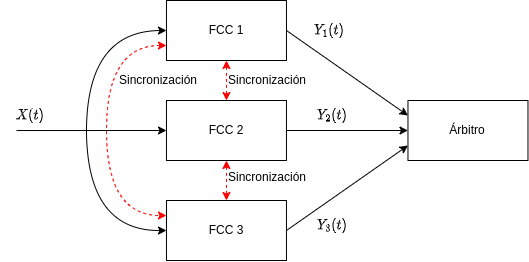
\includegraphics[width=0.7\textwidth]{img/3_4_1_sincronizacion_3.png}
    \caption{La sincronización entre nodos es necesaria para un correcto funcionamiento de las redundancias.}
    \label{fig:3_4_1_sincronizacion_3}
\end{figure}

Se concluye que es mandatorio utilizar alguna técnica de sincronización entre los nodos. Como detalle de la figura \ref{fig:3_4_1_sincronizacion_3}, se muestra que la sincronización entre nodos presupone otro canal de comuniación más. Otra forma podría ser relegar la tarea de la sincronización al bloque \textit{Voter}, aunque esto nuevamente presenta un punto singular de falla. Como se demostró en esta sección, el sincronismo es un aspecto crítico en el sistema redundante, por lo que se prefiere evitar esto último.

\subsubsection{Consenso}

Antes se mencionó que la arquitectura TMR puede mejorarse si se aplica redundancia para los elementos que realizan la votación. En la figura \ref{fig:3_4_2_consenso_1} se muestra la arquitectura TMR con redundancia de elementos que realizan la votación.

\begin{figure}[H]
    \centering
    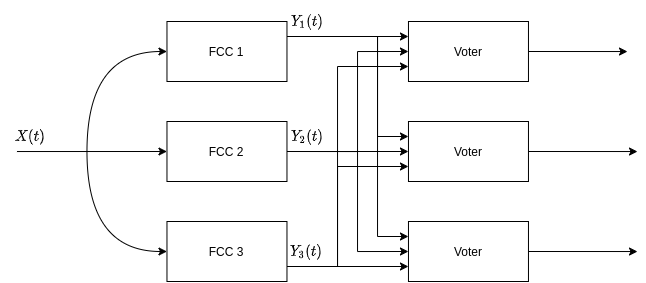
\includegraphics[width=0.7\textwidth]{img/3_4_2_consenso_1.png}
    \caption{Arquitectura TMR con redundancia en los elementos votantes.}
    \label{fig:3_4_2_consenso_1}
\end{figure}

Los tres elementos \textit{Voter} reciben las mismas entradas y deciden un valor. En el caso de que ninguno de los \textit{voters} cometa un error, dado que las entradas de los \textit{Voters} son exactamente iguales, luego los tres decidirán por el mismo resultado como el valor correcto.

Lo que se plantea en esta sección es que existe la posibilidad de que una de las FCC entregue distintos valores a cada \textit{Voter}. En la figura \ref{fig:3_4_2_consenso_2} se muestra una situación en la que la FCC1 entrega dos valores distintos a los demás \textit{Voters}, siendo los valores posibles \textit{True} y \textit{False}. Esto puede deberse por ejemplo a que la FCC1 así lo quiso, debido a una falla muy compleja de analizar y que se manifiesta como un error de esta manera. Otra posibilidad más realista puede ser el hecho de que, debido a que el dato enviado por la FCC1 llegó más tarde al tercer \textit{Voter} que a los demás, este interpretó mal el valor recibido por la línea de comuniación, generando la situación de la figura \ref{fig:3_4_2_consenso_2}. 

\begin{figure}[H]
    \centering
    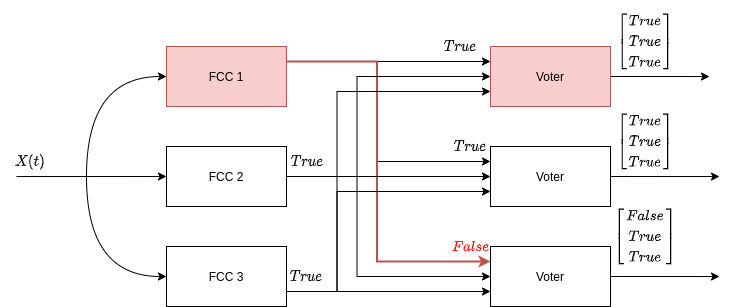
\includegraphics[width=0.8\textwidth]{img/3_4_2_consenso_2.png}
    \caption{La FCC1 entrega el valor de \textit{True} a un \textit{Voter} y \textit{False} a otro. Los vectores representan los valores sobre los que cada \textit{Voter} debe decidir y votar por un único valor.}
    \label{fig:3_4_2_consenso_2}
\end{figure}

Este caso a priori parecería no presentar un problema que la arquitectura TMR no pueda resolver. El primer y segundo \textit{Voter} decidirán por el valor \textit{True}, ya que todas sus entradas son iguales a este valor. El tercer \textit{Voter} también decidirá por el valor \textit{True} ya que 2 de 3 de sus valores son \textit{True}. En definitiva, la arquitectura TMR resuelve el problema del consenso para este caso.

A continuación se plantea un caso diferente. Se analiza la situación en la que cada FCC propone un valor distinto, que fue calculado por su propia observación del escenario en el que se encuentra. Esto podría ser por ejemplo, el valor de algún sensor interno a esta. Las FCC 1, 2 y 3 se encuentran dentro del mismo UAV, por lo que si poseen sensores redundantes, uno esperaría que se obtengan las mismas lecturas (si es que todos los sensores funcionan adecuadamente). Esto puede no ser así, ya que por ejemplo estas pueden presentar pequeñas variaciones por tratarse de lecturas analógicas. De manera de que el algoritmo de control se ejecute de manera consistente en las tres FCCs, ellas deben ponerse de acuerdo en un valor del sensor.

Como se mencionó en la sección anterior, se requiere lograr una sincronización entre computadoras de vuelo redundantes. De manera de ejecutar un algoritmo de sincronización adecuado, las computadoras de vuelo deben compartir un valor asociado a su propio clock interno, a las demás.

Estos dos últmos escenarios difieren del caso en el que la FCC comparte un valor que puede ser \textit{True} o \textit{False}. Lo que se plantea aquí es un caso en el que cada FCC comparte un valor que corresponde a la propia perspectiva de cada una de ellas. Debido a esto, no existe un valor correcto a transferirle a las demás. Se muestra un ejemplo para la sincronización de FCCs en la figura \ref{fig:3_4_2_consenso_4}.

\begin{figure}[H]
    \centering
    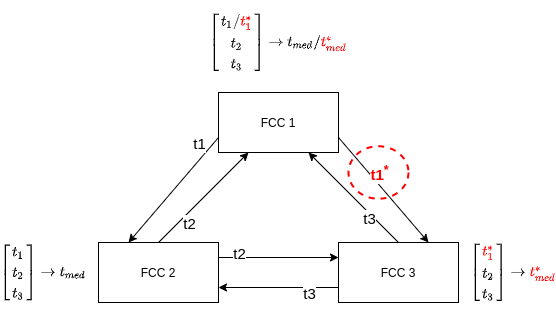
\includegraphics[width=0.6\textwidth]{img/3_4_2_consenso_4.png}
    \caption{La FCC1 entrega un valor distinto de timing a las demás FCCs}.
    \label{fig:3_4_2_consenso_4}
\end{figure}

En este escenario, la FCC1 entrega dos valores distintos de su \textit{clock} a las demás FCCs. Cada una de ellas luego realiza un promedio para llegar a un único valor. Lo que se observa es que las FCC2 y FCC3 calcularán un valor promedio distinto, es decir, no se sincronizarán.
Una posible solución podría ser que las FCCs hagan un nuevo intercambio, con los valores promedio calculados. Esto se muestra en la figura \ref{fig:3_4_2_consenso_5}.

\begin{figure}[H]
    \centering
    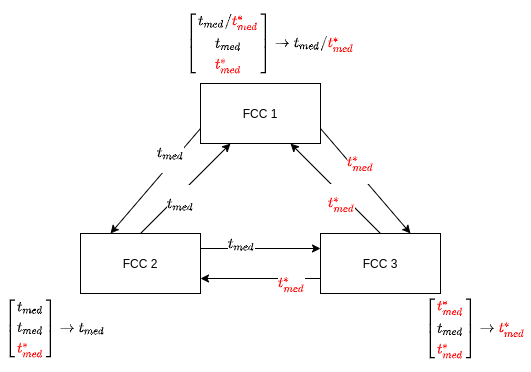
\includegraphics[width=0.6\textwidth]{img/3_4_2_consenso_5.png}
    \caption{Luego de calcular los promedios, las FCCs intercambian sus resultados. Nuevamente, la FCC1 comete una falla en el envío del dato.}
    \label{fig:3_4_2_consenso_5}
\end{figure}

Esta situación puede llevar a que las computadoras de vuelo no se sincronicen, algo que como ya se mencionó, es crítico para la correcta ejecución del algoritmo de tolerancia a fallas.

Podría argumentarse que es demasiado pesimista pensar que la FCC1 puede producir la misma falla 2 veces de manera consecutiva, ya que existe una baja probabilida de que ello suceda.